\documentclass[12pt, a4paper]{article}
\usepackage[spanish]{babel}
\usepackage[utf8]{inputenc}
\usepackage{amsmath}
\usepackage{amsfonts}
\usepackage{amssymb}
\usepackage{graphicx}
\usepackage{hyperref}
\usepackage{algorithm2e}
\usepackage{geometry}
\geometry{left=2.5cm, right=2.5cm, top=2.5cm, bottom=2.5cm}

\title{\textbf{Simulación de Sistema de Mantenimiento de Robots}}
\author{John García Muñoz C-311}
\date{\today}

\begin{document}

\maketitle

\section{Introducción}
\label{sec:introduccion}

\subsection{Descripción del Proyecto}
Se ha escogido el ejrecicio 16, Capítulo 6 del libro Aplicando Teoría de Colas en Dirección de Operaciones (página 59).\\

Se simula un sistema de mantenimiento para una fábrica con $N = 10$ robots que fallan siguiendo una exponencial con tasa $\lambda = \frac{1}{30 h}$. Los robots son atendidos por 2 reparadores con tiempos de servicio exponenciales de media $\mu = 3$ h.\\

\textbf{Nota}: Se ha cambiado el número de robots de 5 a 10 en aras de ofrecer un escenario más interesante.

\subsection{Objetivo}
El objetivo principal es determinar:

\begin{itemize}
    \item Número medio de robots operativos ($L$)
    \item Tiempo promedio en el sistema ($W$)
    \item Porcentaje de inactividad de los reparadores
\end{itemize}

\subsection{Variables de Interés}
\begin{table}[h]
    \centering
    \begin{tabular}{lll}
        \hline
        \textbf{Símbolo} & \textbf{Descripción}\\
        \hline
        $\lambda$ & Tasa de fallos\\
        $\mu$ & Tasa de reparación\\
        $L$ & Robots operativos promedio\\
        $W_q$ & Tiempo en cola promedio\\
        $\rho_1, \rho_2$ & Utilización de reparadores\\
        \hline
    \end{tabular}
    \caption{Tabla de variables del sistema}
    \label{tab:variables}
\end{table}


\section{Detalles de Implementación}

\subsection{Metodología General}
El sistema se modeló como un proceso estocástico de eventos discretos utilizando el paradigma \textit{cola M/M/2 con población finita}. Se implementó en Python con la biblioteca SimPy, siguiendo un enfoque basado en entidades activas (robots) y recursos compartidos (reparadores). La simulación se ejecutó durante 10,000 horas virtuales, descartando las primeras 1,000 horas para eliminar efectos transitorios (siendo muy conservadores, pero no importa ya que se asume que el comportamiento de los robots no se desgasta con el tiempo).

\subsection{Componentes Clave del Modelo}
\begin{itemize}
    \item \textbf{Mecanismo de servicio:} Dos reparadores independientes con tiempos de reparación exponenciales ($\mu = 1/3$ h$^{-1}$). La asignación de robots a reparadores se realiza mediante política aleatoria balanceada.
    
    \item \textbf{Cola de espera:} Estructura FIFO (\textit{First-In, First-Out}) gestionada implícitamente por SimPy al solicitar recursos ocupados.
\end{itemize}

\subsection{Arquitectura de Datos}
\begin{itemize}
    \item \textbf{Registro temporal:} Se almacenaron los tiempos de fallo, inicio/fin de reparación, y estado del sistema cada 0.1 horas.
    
    \item \textbf{Métricas calculadas:} 
    \begin{itemize}
        \item Disponibilidad ($L$): Promedio móvil de robots operativos
        \item Utilización de recursos: Proporción temporal de uso por reparador
        \item Distribución acumulada de tiempos en cola ($W_q$)
    \end{itemize}
    \item \textbf{Exclusión de transitorios:} Se aplicó un período de calentamiento de 1,000 horas para alcanzar el estado estacionario.
\end{itemize}

\subsection{Validación Estadística}
\begin{itemize}
    \item \textbf{Remuestreo bootstrap:} Se generaron 10,000 muestras sintéticas para calcular intervalos de confianza del 95\% en métricas clave.
    
    \item \textbf{Análisis de sensibilidad:} Variaciones controladas de $\lambda$ y $\mu$ para evaluar robustez del modelo.
    
\end{itemize}


\subsection{Integración de Resultados}
Los datos brutos se procesaron mediante un pipeline estadístico en cuatro etapas:
\begin{enumerate}
    \item \textbf{Filtrado:} Eliminación de datos del período transitorio
    \item \textbf{Transformación:} Cálculo de métricas derivadas (ej. $W = W_q + S$)
    \item \textbf{Agregación:} Generación de distribuciones acumuladas y promedios
    \item \textbf{Visualización:} Creación automática de gráficos en Matplotlib
\end{enumerate}

\section{Resultados y Experimentos}
\label{sec:resultados}

\subsection{Hallazgos de la Simulación}
La ejecución de la simulación con 10 robots y 2 reparadores reveló un sistema altamente eficiente pero con capacidad ociosa significativa. Los resultados clave obtenidos fueron:
\begin{itemize}
    \item \textbf{Robots operativos promedio (L):} 9.10
    \item \textbf{Tiempo total en sistema (W):} 3.55 horas
    \item \textbf{Tiempo en cola (Wq):} 0.45 horas (23 minutos)
    \item \textbf{Inactividad de reparadores:} 73.76\% del tiempo total
    \item \textbf{Carga de trabajo:} Reparador 1 (42.70\%) vs Reparador 2 (56.33\%) (% del tiempoque estuvo trabajando)
\end{itemize}

\begin{figure}[h!]
    \centering
    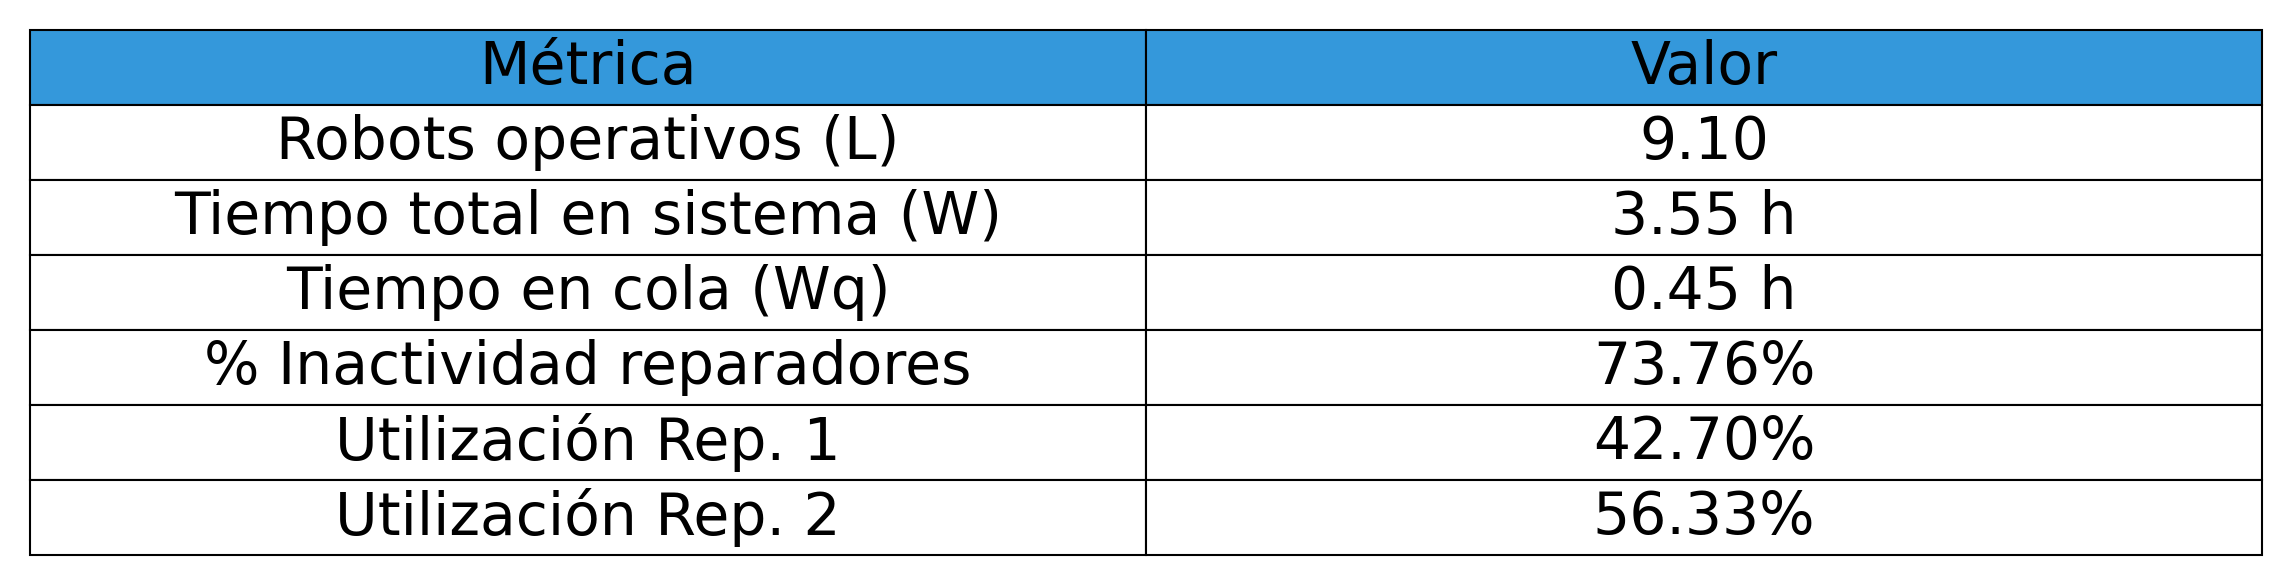
\includegraphics[width=0.8\textwidth]{../img/tabla_resultados.png}
    \caption{Tabla con los resultados}
    \label{fig:ejemplo}
\end{figure}

\begin{figure}[h!]
    \centering
    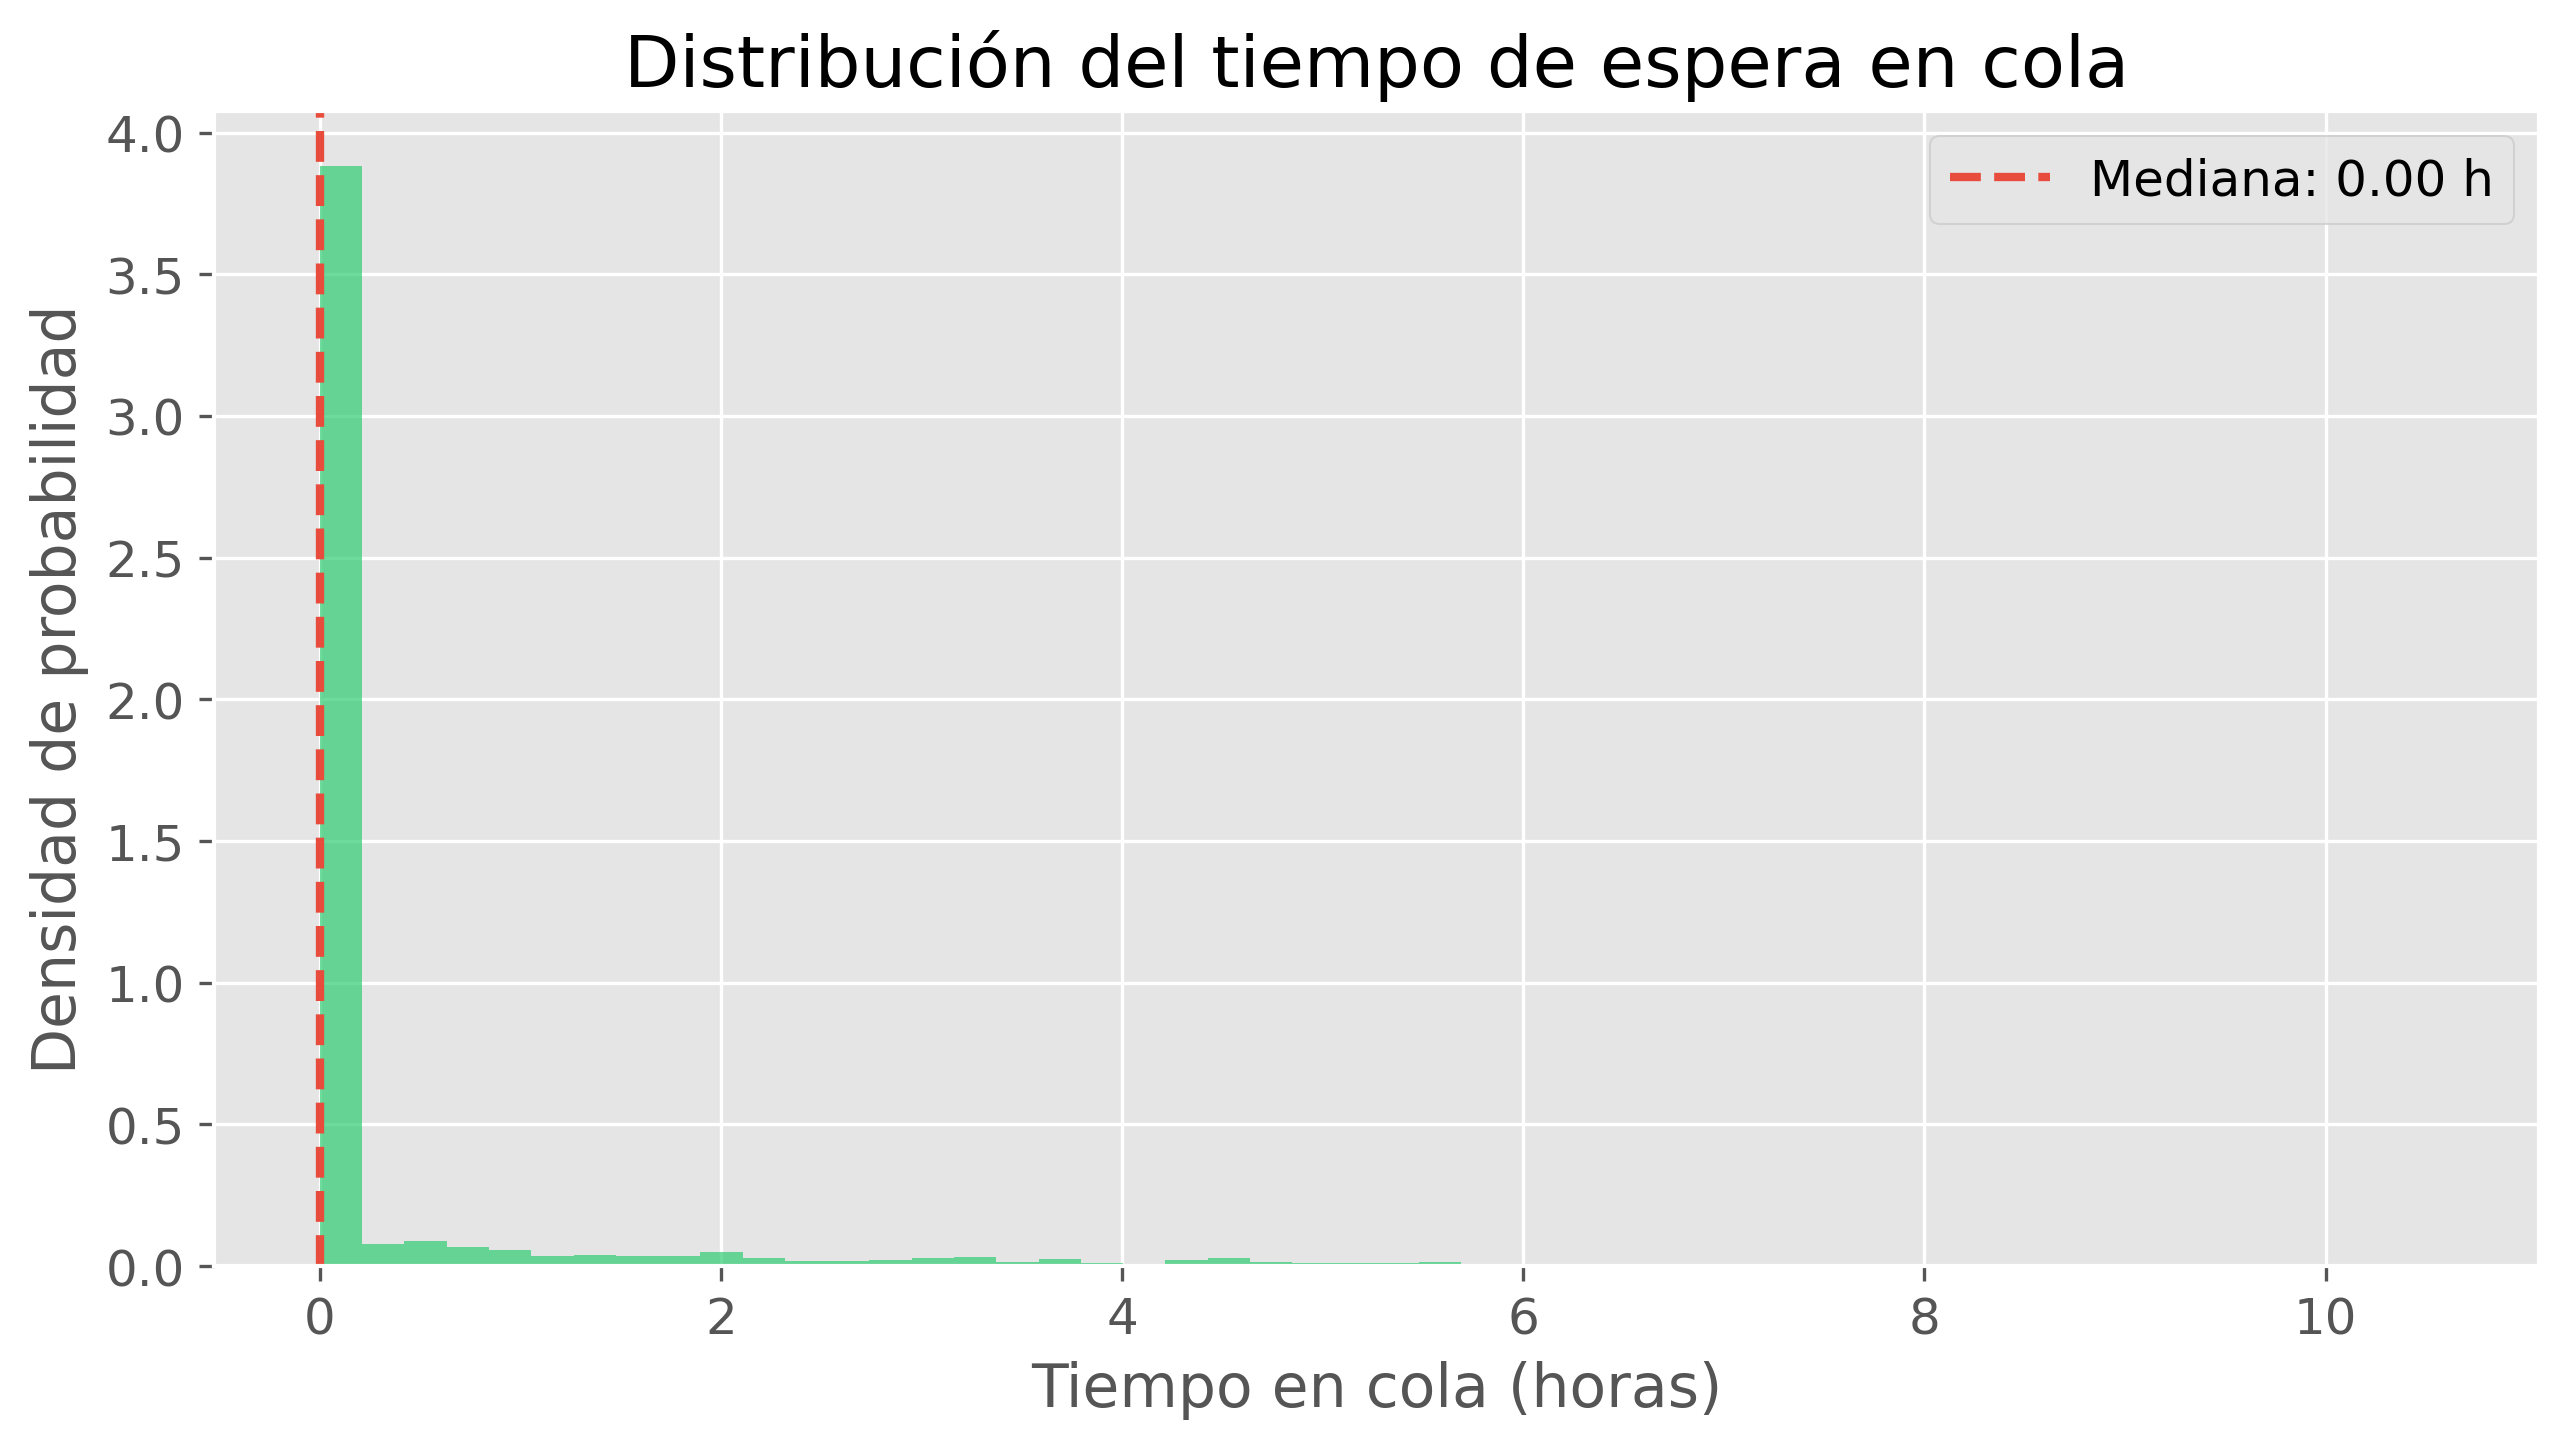
\includegraphics[width=0.8\textwidth]{../img/distribucion_cola.png}
    \caption{Distribución del tiempo de cola}
    \label{fig:ejemplo}
\end{figure}

\begin{figure}[h!]
    \centering
    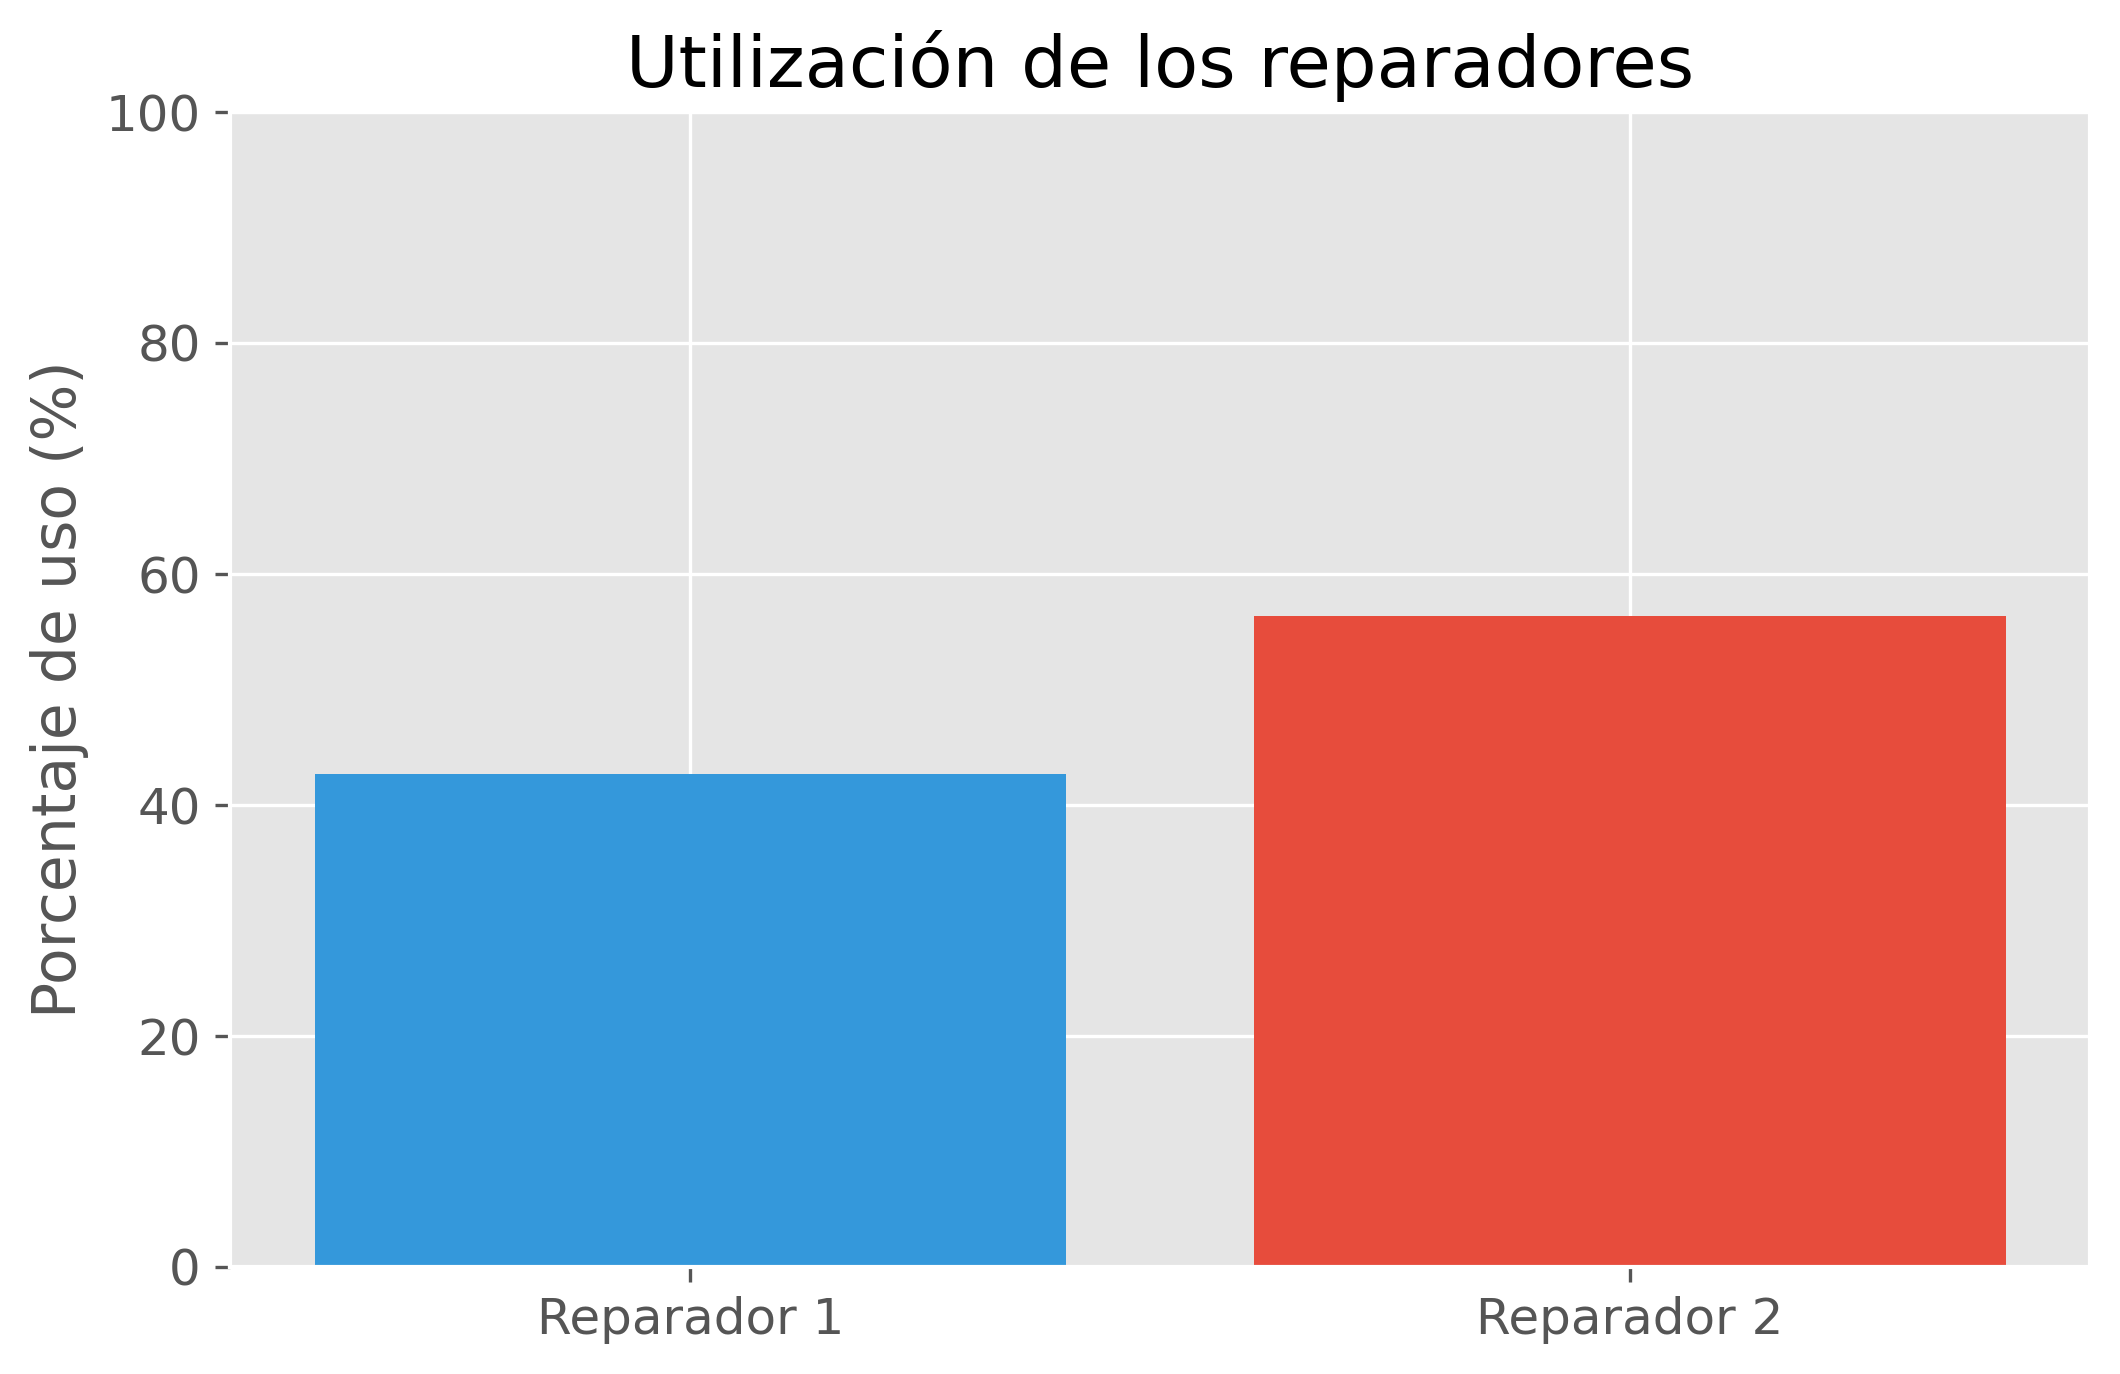
\includegraphics[width=0.8\textwidth]{../img/utilizacion_reparadores.png}
    \caption{\% del tiempo que cada reparador pasó trabajando}
    \label{fig:ejemplo}
\end{figure}

\subsection{Interpretación de los Resultados}
El valor de $L = 9.10$ indica que en promedio menos de un robot (0.9) está fuera de servicio, demostrando alta disponibilidad del sistema. Es difícil que más de un robot estén rotos a la vez. Esto sugiere que dos operarios son suficientes para cubrir la reparación de los 10 robots.

\subsection{Hipótesis Extraída}
\begin{enumerate}
    \item \textbf{Sobrecapacidad:} El sistema podría mantener su eficiencia con un solo reparador.
\end{enumerate}

\subsection{Experimento Realizado}

\textbf{Experimento 1 (Reducción a 1 reparador):}
Tras cambiar el número de reparadores y reducirlo a 1, este pasó a tener una carga de trabajo del 92.55%, lo que representa que en efecto, un reparador puede, técnicamente y en términos de tiempo, encargarse de todos los robots, aunque con poco margn.


\section{Conclusiones}
\label{sec:conclusiones}

\subsection{Hallazgos Principales}
La simulación reveló que el sistema actual con \textbf{10 robots y 2 reparadores} opera en régimen de sobrecapacidad, caracterizado por:
\begin{itemize}
    \item \textbf{Alta disponibilidad}
    \item \textbf{Baja congestión}
    \item \textbf{Alto tiempo de ocio de los trabajadores}
\end{itemize}

    Reducir a un solo operador podría tampoco ser solución, ya que no contaría con mucho margen (ya sea para descanso, o para emergencias).

\begin{center}
\fbox{
\parbox{0.9\textwidth}{
\textbf{Conclusión Final:} \\ 
El sistema actual es \textit{eficiente pero ineficaz} — si bien garantiza alta disponibilidad, desperdicia un gran tiempo de la capacidad de reparación. Una política híbrida con 1 reparador full-time y otro parcial reduciría costos y mantendría una postura suficientemente conservadora.
}}
\end{center}

\end{document}